\documentclass[10pt, a4paper]{jsarticle}
\title{モンテカルロ木探索における\\シミュレーションのGPUを用いた並列化}
\author{明治大学理工学部情報科学科\\知的情報処理システム研究室\\4年15組28番 高野昂平}
\date{}

\usepackage[dvipdfmx]{graphicx}

\begin{document}
\maketitle
% \tableofcontents
\newpage
\section{はじめに}
\subsection{研究概要}
モンテカルロ木探索(Monte Carlo Tree Search, MCTS)におけるシミュレーション部分を並列化し、高速化を目指す。
オセロを対象に実験を行った。
\subsection{研究背景}
モンテカルロ木探索の処理速度向上を図るうえで、シミュレーション部分が全体の処理速度のボトルネックとなっているのではと考え、シミュレーション部分を並列化することが全体の高速化につながるのではないかと考えた。\par
高性能なCPUを用いることで高速化を図ることも考えられるが、近年CPUの性能向上率が以前に比べて伸び悩んでおり、高速化を図るためにはCPUに依存した手法では高止まりになってしまう。そこで、別のアプローチで高速化を目指す必要があるが、その手法としてGPUを用いた並列化を選択した。近年、GPUを画像処理だけでなく、汎用計算に用いてGPGPU(Generarl Purpose GPU)として活用する動きも見られるため、モンテカルロ木探索に対してもGPGPUとして活用できないものかと考えた。
\section{関連研究}
\section{モンテカルロ木探索について}
本研究のテーマであるモンテカルロ木探索(Monte Carlo Tree Search, MCTS)とは、乱数を用いた計算手法であるモンテカルロ法を木探索に応用した手法である。
\par まず、評価関数を用いないという特徴を持つため、様々なゲームのプレイヤーに対してモンテカルロ木探索を実装することができる。例えば、General Game Playing(GGP)という汎用ゲームに対して人間の介入なしで強いプレイヤーを作るという試みがあるが、そのプレイヤーとしてモンテカルロ木探索を用いることが可能である。
\par また、不要な探索を行わないという特徴を持つ。合法手が膨大なゲームに対して木探索を行う場合、そのすべてのノードを探索することによって強いプレイヤーの作成するのは計算量が多くなってしまい、現実的でない。例えば、本研究ではオセロのプレイヤーに対して、モンテカルロ木探索を施したが、そのオセロの合法手は$10^{28}$手あると推測されており、すべてのノードを探索することが困難であることがわかる。しかし、モンテカルロ木探索の場合、すべてのノードを探索するのではなく、有効と考えられる手を優先的に深く探索するため、無駄な探索をすることがなく、計算量を削減することができる。
\par モンテカルロ木探索の流れとしては、選択、シミュレーション、展開、逆伝播の4ステップからなっており(図\ref{fig:parallel})、本研究では2ステップ目のシミュレーションを並列化することを目標としている。
\subsection{UCTについて}
選択ステップにおいて、次に訪問するノードを決めるアルゴリズムとして、UCTアルゴリズムを採用した。このアルゴリズムは、以下の式が最大となるようなノードを次の訪問ノードとするアルゴリズムである。
\par 以下の式において、$w$はそのノードにおける評価値、$n$はそのノードにおける訪問回数、$N$はそのノードを親としたと きの子ノードの$n$の値の合計値、$C$は任意の値で探索がうまくいくように調整すべきパラメータとなっている。
\begin{eqnarray}
    UCT = \frac{w}{n} + C\sqrt{\frac{\ln{N}}{n}}
\end{eqnarray}
\par
この式が意味するのは、ノードの評価値だけで訪問先を決めるのではないということで、第1項自体は評価値の平均を取っているが、第2項において訪問回数が少ないノードを訪問するようにUCT値を調整しているのがわかる。変数$C$はこの訪問回数の少ないノードへの訪問をどれくらい重く見るべきか定めるパラメータと言える。
\subsection{並列化手法}
本研究では、シミュレーション部分を並列化するが、具体的には以下の図\ref{fig:parallel}のように、4ステップあるモンテカルロ木探索の2ステップ目を複数回のシミュレーションを同時に実行することで実現する。
\begin{figure}[ht]
    \begin{center}
        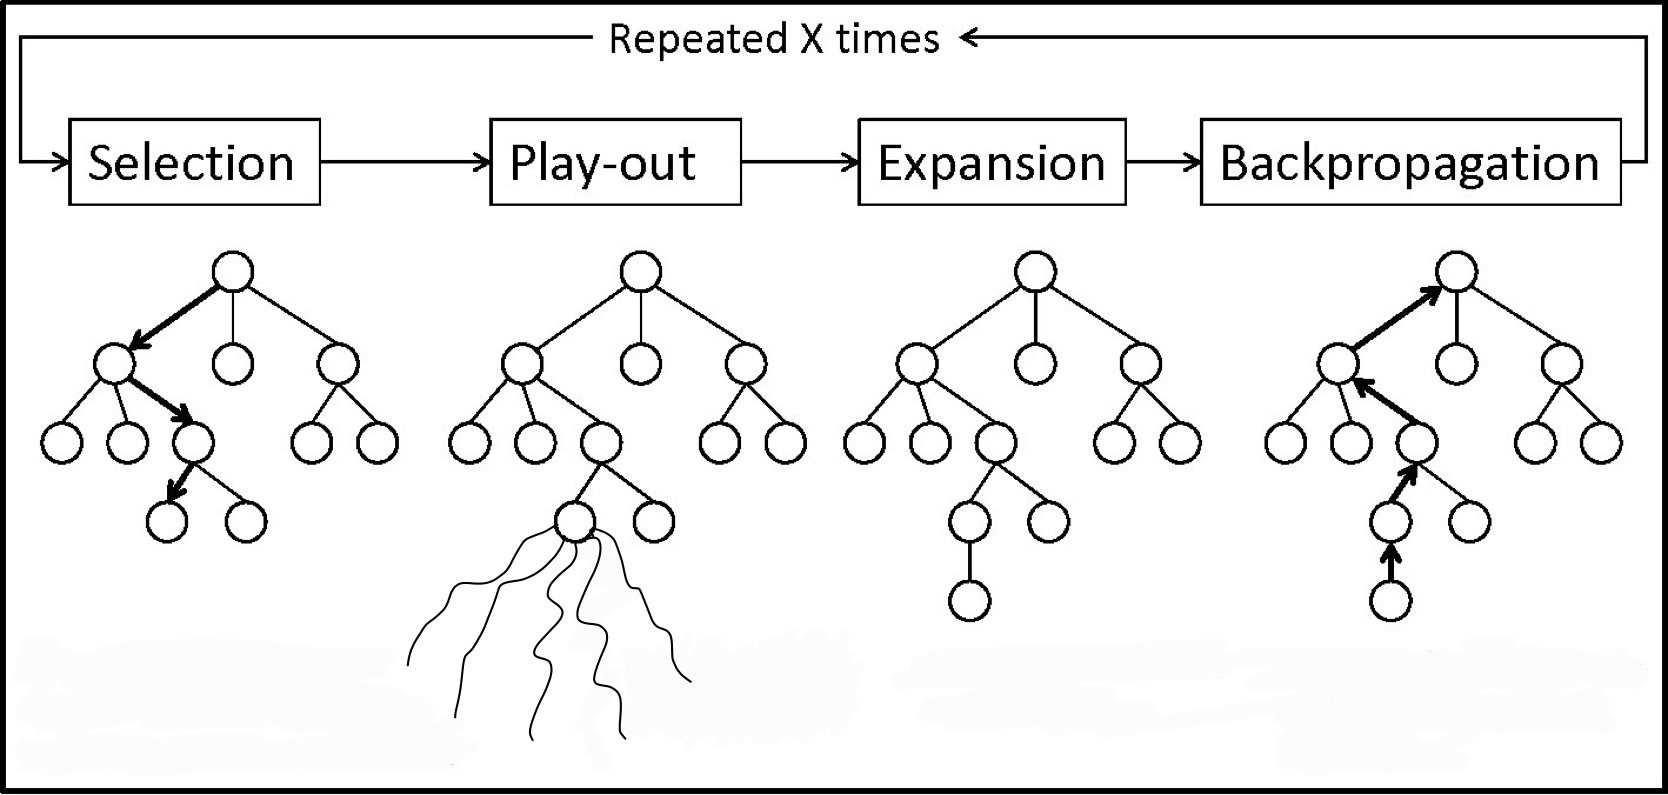
\includegraphics[width=15cm]{img/mcts_parallel.jpg}
        \caption{シミュレーションの並列化} \label{fig:parallel}
    \end{center}
\end{figure}
\par 複数回のシミュレーションを行う際、CPUでの逐次実行とGPUでの並列実行の違いは、まず、逐次実行の場合には図\ref{fig:cpu_mcts_code}のように1回のシミュレーションをfor文によって複数回順番に実行し、それぞれのシミュレーションをで得た値を足し合わせることで処理を行っている。
\par 一方、並列実行の場合、図\ref{fig:gpu_mcts_code}のように1回のプレイアウト関数の呼び出しによって、複数回のシミュレーションを終えている。厳密には、playout\_cuda関数内でのカーネル呼び出しによって並列にシミュレーションが行われる。
\begin{figure}[ht]
    \begin{center}
        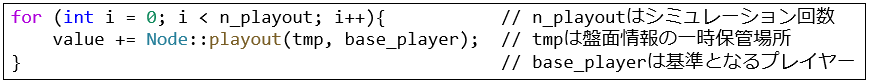
\includegraphics[width=15cm]{img/cpu_mcts_code.png}
        \caption{CPUによる逐次実行}
        \label{fig:cpu_mcts_code}
    \end{center}
\end{figure}
\begin{figure}[ht]
    \begin{center}
        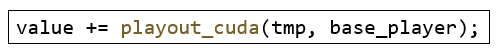
\includegraphics[width=12cm]{img/gpu_mcts_code.png}
        \caption{GPUによる並列実行}
        \label{fig:gpu_mcts_code}
    \end{center}
\end{figure}
\section{実験環境}
\subsection{パラメータについて}
ある盤面ノードに対する評価回数(図\ref{fig:parallel}におけるX)を100回、ノードの展開の基準値を20回訪問とした。また、CUDAカーネルを1ブロックあたりのスレッド数を512として、実験を行った。
\subsection{並列化環境について}
並列化にあたって、NVIDIA社のCUDA(Compute Unified Device Architecture)を用いた。CUDAはNVIDIA社のGPU上で動作する汎用並列コンピューティングプラットフォームである。なお、言語はC++とし、CUDA Cを用いて実装を行った。
\subsection{実行環境}
CUDAを用いる関係上、GPUはNVIDIA社のものとなっている。
\begin{table}[ht]
    \begin{center}
        \begin{tabular}{ll}
            OS & Ubuntu 20.04.2 LTS \\
            CPU & Intel(R) Core(TM) i9-10900X CPU @ 3.70GHz \\
            GPU & GeForce RTX 3080 (CUDAコア 8704)\\
            メモリ & 32GB \\
        \end{tabular}
    \end{center}
\end{table}
\section{実行速度の計測}
\subsection{実験概要}
実験の流れとしては、オセロの初期盤面における評価(図\ref{fig:parallel}における1サイクル)を100回行う。それぞれの評価を行う中で、CPUでのシミュレーションとGPUでのシミュレーションを実行する。各シミュレーションで実行時間を計測し、100回分の実行時間を計測し終わった後、それらの平均を求める。この平均をもとに実行時間の比較を行った。
\subsection{実行時間の比較}
\begin{figure}[ht]
    \begin{center}
        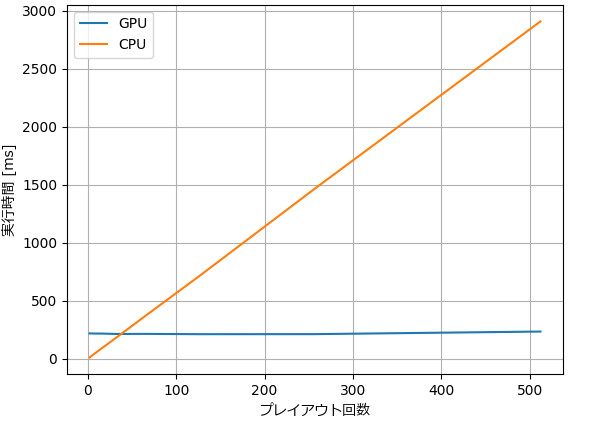
\includegraphics[width=12cm]{img/gpu_cpu_time.png}
        \caption{実行時間の比較}
        \label{fig:cpu_gpu_time}
    \end{center}
\end{figure}
\par 図\ref{fig:cpu_gpu_time}はプレイアウト数を1から順に2倍ずつ増やしたときの、実行時間の変化をグラフにしたものである。
\par 図\ref{fig:cpu_gpu_time}からわかるように、CPUの逐次実行での実行時間が線形的に増加しているのに対して、GPUでの実行時間は並列処理であるため、実行時間が増えていない。
\par しかし、CUDAコア数以上の並列数(プレイアウト数)で実行するとすべてのプレイアウトを同時に処理できず、並列処理自体を順次実行していくため、実行時間が増加していく。これについては後述する。
\subsection{並列処理の実行時間の増加について}
\begin{figure}[ht]
    \begin{center}
        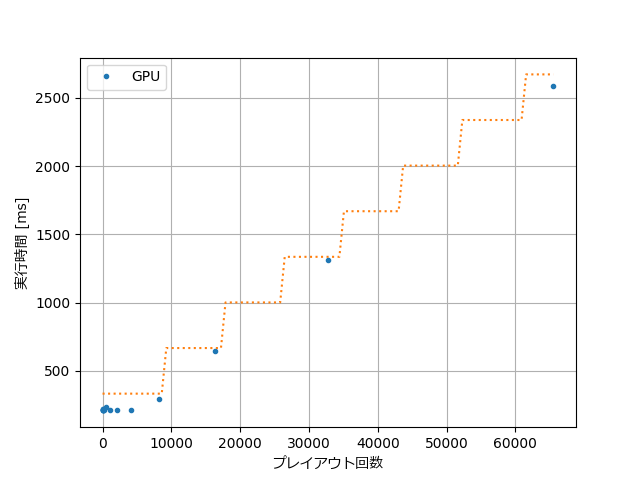
\includegraphics[width=12cm]{img/gpu_time_wCeil.png}
        \caption{GPUでの実行時間}
        \label{fig:gpu_time}
    \end{center}
\end{figure}
\par 図\ref{fig:gpu_time}は、さらにプレイアウト数を増やした場合のGPUでの実行時間の変化をグラフにしたものである。本実験ではプレイアウト数を2倍ずつ増やしているため、その実行時間をグラフにした際に、線形的に増加しているように見える。しかし、プレイアウト数を細かく変化させ、実行時間を計測した場合、天井関数に近い形のグラフになることが予想される。予想される天井関数の概形が図\ref{fig:gpu_time}における点線部分にあたる。
\par 並列に実行した場合でも、プレイアウト数を増やしていくとCPUでの逐次実行と同様に実行時間が増えていくことがグラフから見て取れるが、しかし、その増加幅はCPUでの逐次実行に比べて緩やかなものとなっており、このままプレイアウト数を増やしたとしても、並列処理での実行時間の短縮は実現できるものと考える。
\section{強さの比較}
\subsection{実験概要}
強さの比較を行うにあたって、先手黒の強さのプレイアウト回数を大きくしていくことで検証を行った。また、後手白の強さはプレイアウト回数を2048回とした。
\subsection{t検定}
本実験を行う上でt検定を行い、勝率を評価した。帰無仮説を"先手黒と後手白の強さは同じ"とし、また、対立仮説を"白が黒より強い"とした。対立仮説をこのようにしたのは、今回の実験において、後手白のプレイアウト回数が先手黒のプレイアウト回数より多いことが保証されており、白の強さが黒を下回ることは予想されないためである。この対立仮説を示すために、片側検定を行った。よって、有意水準を0.05としたとき、z値が-1.64を下回る勝率に関しては、帰無仮説が棄却され、対立仮説を採用するため"白が黒より強い"ということが有意に言える。
\subsection{勝率の評価}
\begin{table}[ht]
    \begin{center}
        \begin{tabular}{c|c|c|c|c}
            プレイアウト数 & 勝ち数 & 負け数 & 勝率[\%] & z値 \\ \hline
            1 & 4 & 146 & 2.67 & -11.59 \\
            2 & 18 & 131 & 12.08 & -9.26 \\
            4 & 27 & 120 & 18.37 & -7.67 \\
            8 & 36 & 113 & 24.16 & -6.31 \\
            16 & 55 & 94 & 36.91 & -3.2 \\
            32 & 65 & 84 & 43.62 & -1.56 \\
            64 & 64 & 82 & 43.84 & -1.49 \\
            128 & 81 & 69 & 54.00 & 0.98 \\
            256 & 74 & 72 & 50.68 & 0.17 \\
            512 & 67 & 81 & 45.27 & -1.15
        \end{tabular}
        \caption{勝率}
        \label{tab:win_rate}
    \end{center}
\end{table}
\par 表\ref{tab:win_rate}より、プレイアウト回数を1回のとき、先手黒が後手白より圧倒的に弱いことがわかる。徐々にプレイアウト回数を増やしていくと後手白の強さに近づいていくことがわかる。特に、プレイアウト回数128回及び256回では、先手黒のプレイアウト回数が後手白よりも少ないにもかかわらず勝ち越しているため、ある程度のプレイアウト回数があれば、それ以上増やしても強さに大きな影響はないといえる。
\section{終わりに}
\end{document}